The artificial neural network is a potent machine learning modelling method. Our empirical analysis employs a simple feed-forward neural network architecture. The input layer comprises a set of firm-specific and macroeconomic variables. One or more hidden layers capture interactive effects among different variables and perform non-linear transformations on the input variables. The output layer aggregates all the information from the last hidden layer to generate the ultimate prediction output. This can be demonstrated by figure \ref{fig: ff-neural network},

\begin{figure}[H]
  \centering
  \caption{\textbf{Demonstration of Feedforward Neural Network with One Hidden Layer}}
  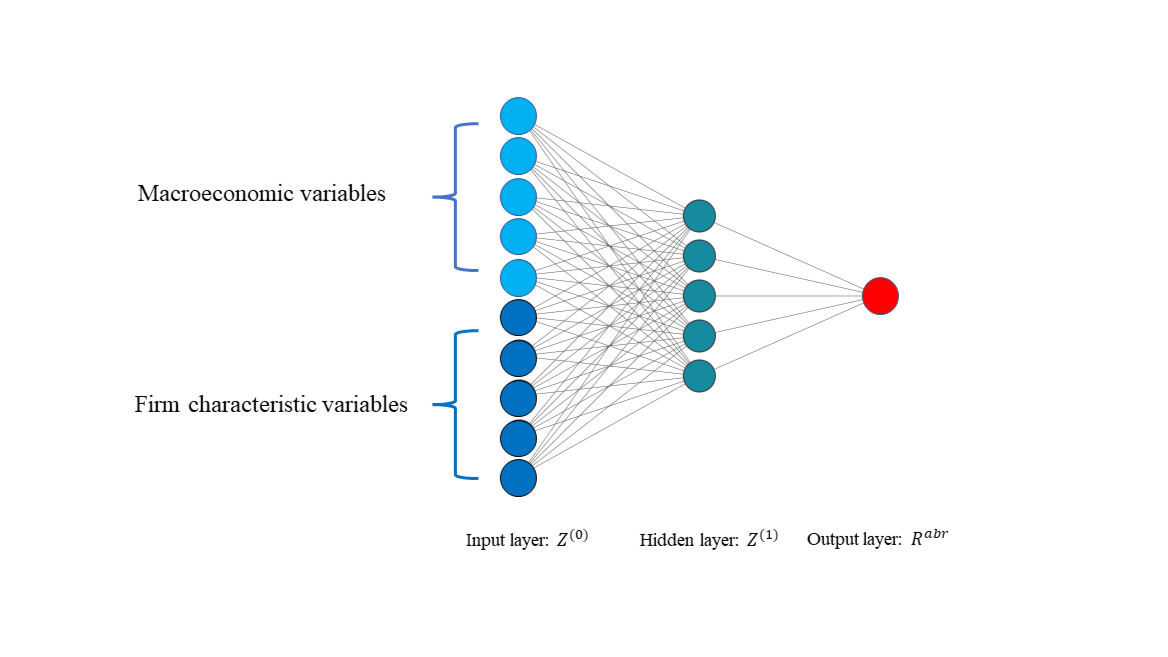
\includegraphics[width=.8\textwidth]{images/fnw_demonstration.png}
  \label{fig: ff-neural network}
\end{figure} 

As posited by \citet*{gu2020empirical}, the stock return can be described using an additive prediction error model as shown below:

\begin{equation}
\label{eqn: generalized model}
R^{abr}_{i,t+1} = E_t(R^{abr}_{i,t+1}) + \epsilon_{i,t+1}
\end{equation}

Here, $E_t(R^{abr}_{i,t+1}) = g(z;\theta)$, where stocks are indexed as $i=1,2,...,N$ and months are indexed by $t=1,2,...,T$. The function $g(z,\theta)$ denotes a mapping function with a set of predictors $z$ and a set of parameters $\theta$, which correspond to the weights and bias in each layer of the neural network model. Through a feed-forward neural network, the model learns to map the inputs to the outputs by adjusting the weights of each layer in response to the errors the model makes on the training dataset. This can be expressed mathematically as follows:
\begin{equation}
  \label{eqn:update weights}
  g(z;\theta) = \theta_0 + \sum^n_{j=1}x_j\theta_j
  \end{equation}

\subsection{Objective Function}

Due to the high number of unknown parameters, obtaining the perfect weights for a neural network model is impossible. Instead, the objective can be reformulated as an optimization or searching problem, where the algorithm aims to find a set of weights that enables the model to make accurate predictions. The commonly used algorithm for training the neural network model is stochastic gradient descent (SDG), which updates the weights using the backpropagation of errors method. Initially, the model makes predictions using the initial weights, and the error is then calculated based on those predictions. The gradient descent algorithm is then used to adjust the weights so that the prediction error is minimized, see an exhaustive discussion by \citet*{domingos2012few}. Mean squared error (MSE) and mean absolute error (MAE) are common objective functions (i.e. loss functions) used in training the neural network model. However, in our study, since there are significant outliers in the abnormal return data, we followed the convention in empirical asset pricing by choosing MSE as the objective function.

\subsection{Activation Function}

Activation functions are a critical component in neural network construction. The choice of activation function in the hidden layer determines how the weighted sum of inputs is transformed into an output from the previous layer to the next, while the choice of activation function in the final output layer determines the type of prediction the model will make. There are various potential choices for the activation function, such as softmax, sigmoid, and ReLu. The architecture of the neural network model ensures that the interaction effect within different variables is captured, while the proper choice of activation function guarantees that the non-linear impact of individual predictors on expected returns is also taken into account. In this study, a linear function is chosen as the final output activation function because the stock returns being predicted are rather random and contain extreme values. Introduced by \citet*{nair2010rectified}, ReLu is selected as the activation function for each hidden layer due to its simplicity, computing advantages, and following the convention in existing literature. ReLu is a piecewise linear function with two linear pieces that will output the input directly if it is positive; otherwise, it will output zero. It is defined as:

\begin{equation}
  \label{eqn:ReLU}
  ReLU(x) = \begin{cases}
    0 & if \ x < o \\
    x & otherwise,
  \end{cases}
  \end{equation}

\subsection{Learning Rate}

The learning rate is a crucial hyperparameter in neural networks as it governs the magnitude of change to the model during each step of the weight updating process. By controlling the speed of learning, the learning rate is a key factor in determining the performance of the model. When the learning rate is set to a high value, the model is able to learn quickly, but yeild a not so accurate prediction; conversely, a low learning rate can enable the model to reach an optimal, or even globally optimal, set of weights, albeit at the cost of a significantly longer training time. The learning rate typically takes a value in the range of 0 to 1. However, an excessively large learning rate may cause the model's performance to oscillate in each training epoch, resulting in divergent results. Conversely, an overly small learning rate may never converge or become trapped in a suboptimal solution.

To accelerate the model training process and optimize the weight searching procedure, we follow \citet*{smith2017cyclical} and introduce momentum to the learning process and utilize a learning rate schedule. Specifically, we incorporate an exponentially weighted average of prior updates into the next update, allowing previous updates in one direction to continue in that direction in the future. Momentum is independent of the choice of learning rate but can enhance the speed of the optimization process when used in combination with the learning rate, increasing the likelihood of finding an optimal set of weights in fewer training epochs. Instead of utilizing a constant learning rate, we vary the learning rate during the training process, referred to as a learning rate schedule or learning rate decay. The fundamental concept is to employ a larger learning rate at the outset to expedite the training process, and gradually reduce the learning rate as the training epochs progress. This approach avoids oscillating model performance and becoming trapped in suboptimal solutions, or failing to converge entirely. A commonly used formula for the learning rate schedule is shown in Equation \ref{eqn:learningrate}:

\begin{equation}
  \label{eqn:learningrate}
  Learning \ Rate = Initial \ Rate * \frac{1}{1 + decay * iteration}
  \end{equation}

\noindent In comparison with a fixed learning rate, utilizing a learning rate schedule can reduce sensitivity to the initial learning rate and provide improved performance. The selection of the learning rate can be visualized through a plot of the changing pattern, as shown in Figure \ref{fig: learningrate}.

\begin{figure}[H]
  \centering
  \caption{\textbf{Learning Rate Scheduale}}
  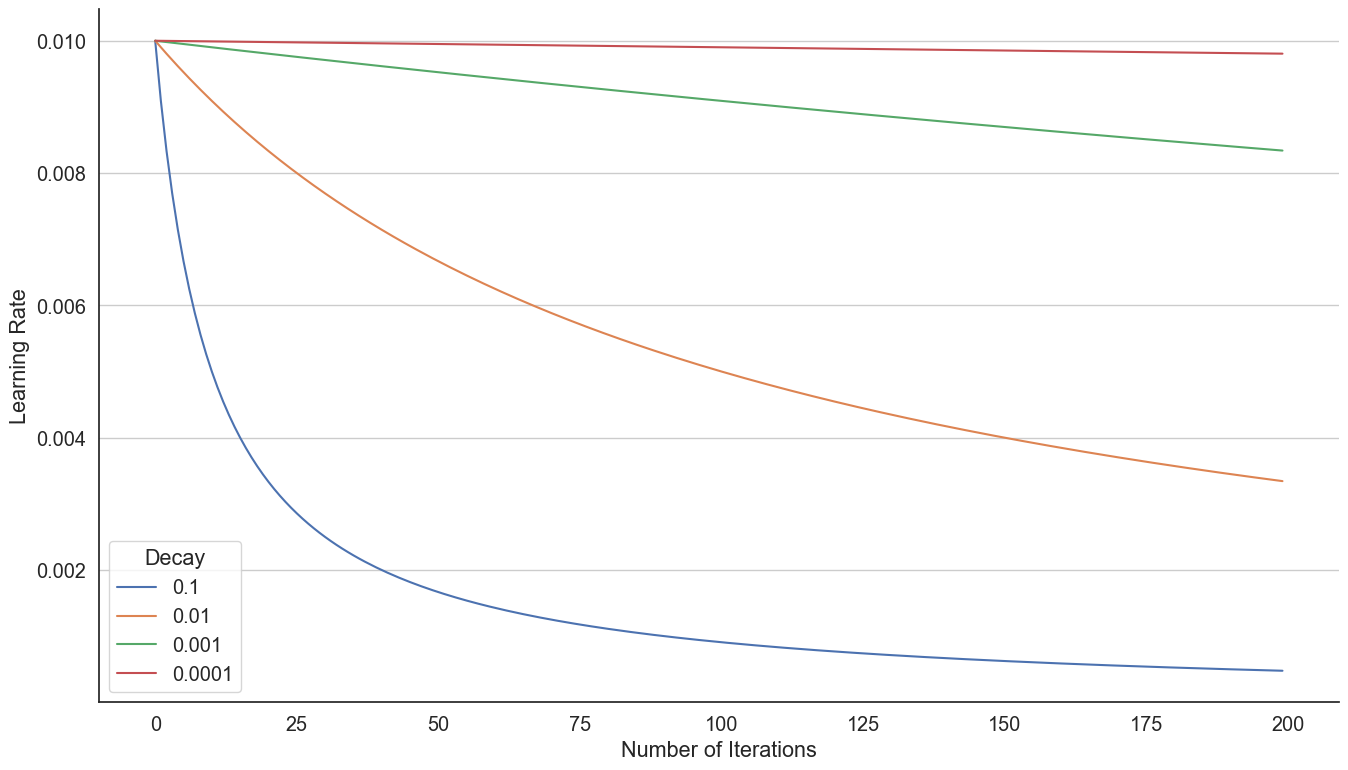
\includegraphics[width=.8\textwidth]{images/learning rate decay.png}
  \label{fig: learningrate}
  \caption*{\footnotesize{This graphic shows a basic learning rate schedule with different decay rates.  The initial learning rate is 0.01, and along with the increasing number of iterations the learning rate starts to decrease to achieve a state of art accuracy.}}
\end{figure}

\subsection{Fix Overfitting with Regularization}

Overfitting is one of the most significant challenges associated with neural network models, where the model performs exceptionally well on the training data but poorly on the test data. The objective of machine learning is to enable the model to learn from example data and generalize to explain new data in the future; however, an overfitted model cannot accomplish this goal. Various regularization techniques discussed by \citet*{tian2022comprehensive}, including activity regularization, weight constraints, dropout, and noise addition, can be employed to combat overfitting. Of these methods, weight regularization is the most widely used. When a model is fitted with sufficient epochs, the weights can become highly specialized to the training data and lead to overfitting. The weights increase in magnitude to capture the specifics of the training data, but this can cause instability in the model and poor performance in predicting test data due to minor variations. Weight regularization imposes a penalty on the model during training based on the magnitude of the weights, with the objective of keeping the weights small. In this paper, we apply an $L1$ penalty (Lasso) to the network weights to promote sparsity.

\subsection{Improve Prediction with Ensembles}

Neural networks can be highly sensitive to the initial conditions, including the random weights and the specific characteristics of the training data. As a result, different initial conditions can lead to the discovery of different sets of weights, and the model can make different predictions when fed with new input data. To address this issue, a common approach is to train multiple models and combine their predictions to ensure a more stable and accurate final prediction. While combining different models can introduce some bias, it can also alleviate the high variance problem caused by a single model. This approach is commonly referred as ensembled learning. There are multiple ensemble learing methods discussed by \citet*{sagi2018ensemble}, among which we use the simplest method to aggregate 10 neural network models to get robust results.

\subsection{Other Model Settings}

The batch size plays a crucial role in training neural network models, impacting both the prediction accuracy and computational efficiency. It represents the number of training samples used per iteration in the training process. A larger batch size leads to a more accurate estimation as more training samples are used, increasing the likelihood of navigating the weight search towards optimal performance. However, smaller batch sizes can result in noisy weight updates, leading to more robust models in some cases. Therefore, the choice of batch size can affect the accuracy of the estimation, the stability of the learning process, and the speed at which the model learns. Consequently, selecting an appropriate batch size is a trade-off between these factors. As a result, the batch size is a critical hyperparameter in the learning algorithm that requires tuning to optimize the model's performance. \citet*{ioffe2015batch} apply batch normalization method to normalizes the activations of each layer in the network over the mini-batch of samples. They show that Batch Normalization can significantly accelerate the training of deep neural networks by reducing the internal covariate shift problem.

In the context of neural networks, the initialized weights of a model are typically small random variables that are updated during the training process using an optimization algorithm. To generate the initial weights, the He initializer proposed by \citet*{he2015delving} is commonly used. In addition to the initialization of weights, the scale of input and output variables can also have a significant impact on the training process and the resulting model performance. To address this, we used a standardized scaler on the training dataset, which was then applied to both the validation and test datasets. This approach helped to speed up and stabilize the training process, and ensured that the model was able to learn effectively from the available data.

\subsection{Feature Importance}
\label{subsec:feature importance}

While deep learning models have powerful predicting ability, there are still criticisms that claim that methods such as neural networks lack interpretability, and that the models used are more like a "black box". Therefore, correctly interpreting the predicted output is equally as important as the predicting accuracy, as it can provide insights into how the output is influenced by variables, give insights into how a model can be improved, and help understand how the process is being modeled. In this paper, we use SHAP values, as described by \citet*{NIPS2017_8a20a862}, to measure feature importance. SHAP (SHapley Additive exPlanation) values track the change in the predicted outputs made by the model by conditioning on each specific feature. They use additive feature attribution methods, with the following mathematical expression, but replace $f(x)$ with $f_x(z')=f(h_x(z'))=E[f(z)|z_s]$:

\begin{equation}
  \label{eqn:shap}
  f(x)=g(x')=\phi_0+\sum^M_{i=1}\phi_i x'_i
  \end{equation}

The explanation model $g(x')$ is designed to match the original model $f(x)$, where $x = h_x(x')$. In this framework, $\phi_0 = f(h_x(0))$ represents the model output with all simplified inputs dropped off (i.e., missing). The $s$ in $E[f(z)|z_s]$ refers to the set of non-zero indexes in $z'$. If an observation has an actual output value of 0 (the base value), some features may push the predicted output away from the actual value, while other features may pull it back closer to the actual value. The final predicted output $f(x)$ can be seen as the balance of power, as illustrated in Figure \ref{fig: shap_demo}. The SHAP values track the change in the predicted output made by the model conditioning on each specific feature and use an additive feature attribution method, as expressed in the mathematical formula provided earlier in Equation \ref{eqn:shap}.

\begin{figure}[H]
  \centering
  \caption{\textbf{SHAP Value Demonstration}}
  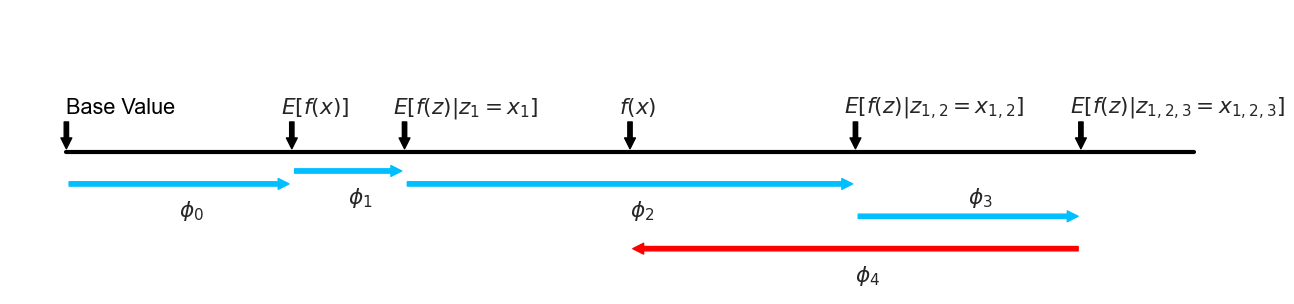
\includegraphics[width=.9\textwidth]{images/shap_force_dem.png}
  \label{fig: shap_demo}
\end{figure}

